\section{Background}
\label{sec:03_background}

\subsection{Group of Pictures Structure}
\label{subsec:subsec_31_gop}
Modern video compression standards such as H.264 and H.265 organize video content through inter-frame dependency structures designed to reduce temporal redundancy. Based on their coding dependencies, video frames are divided into three types: I-frames (intra-coded frames), P-frames (predictive frames), and B-frames (bi-predictive frames). I-frames are encoded independently without reference to any other frame and therefore capture complete spatial scene information. P-frames encode differences relative to preceding reference frames, while B-frames reference both past and future frames for higher compression efficiency. These complementary frame types are organized into a periodic structure known as a Group of Pictures (GOP). As illustrated in Fig.~\ref{fig:fig02_gop_structure}, each GOP begins with an I-frame and encompasses all subsequent P-frames and B-frames up to, but not including, the next I-frame. A key property of the GOP structure is that inter-frame dependencies are typically confined within GOP boundaries, making each GOP a relatively self-contained spatio-temporal unit with strong internal semantic and temporal coherence.

\begin{figure}[!t]
\centering
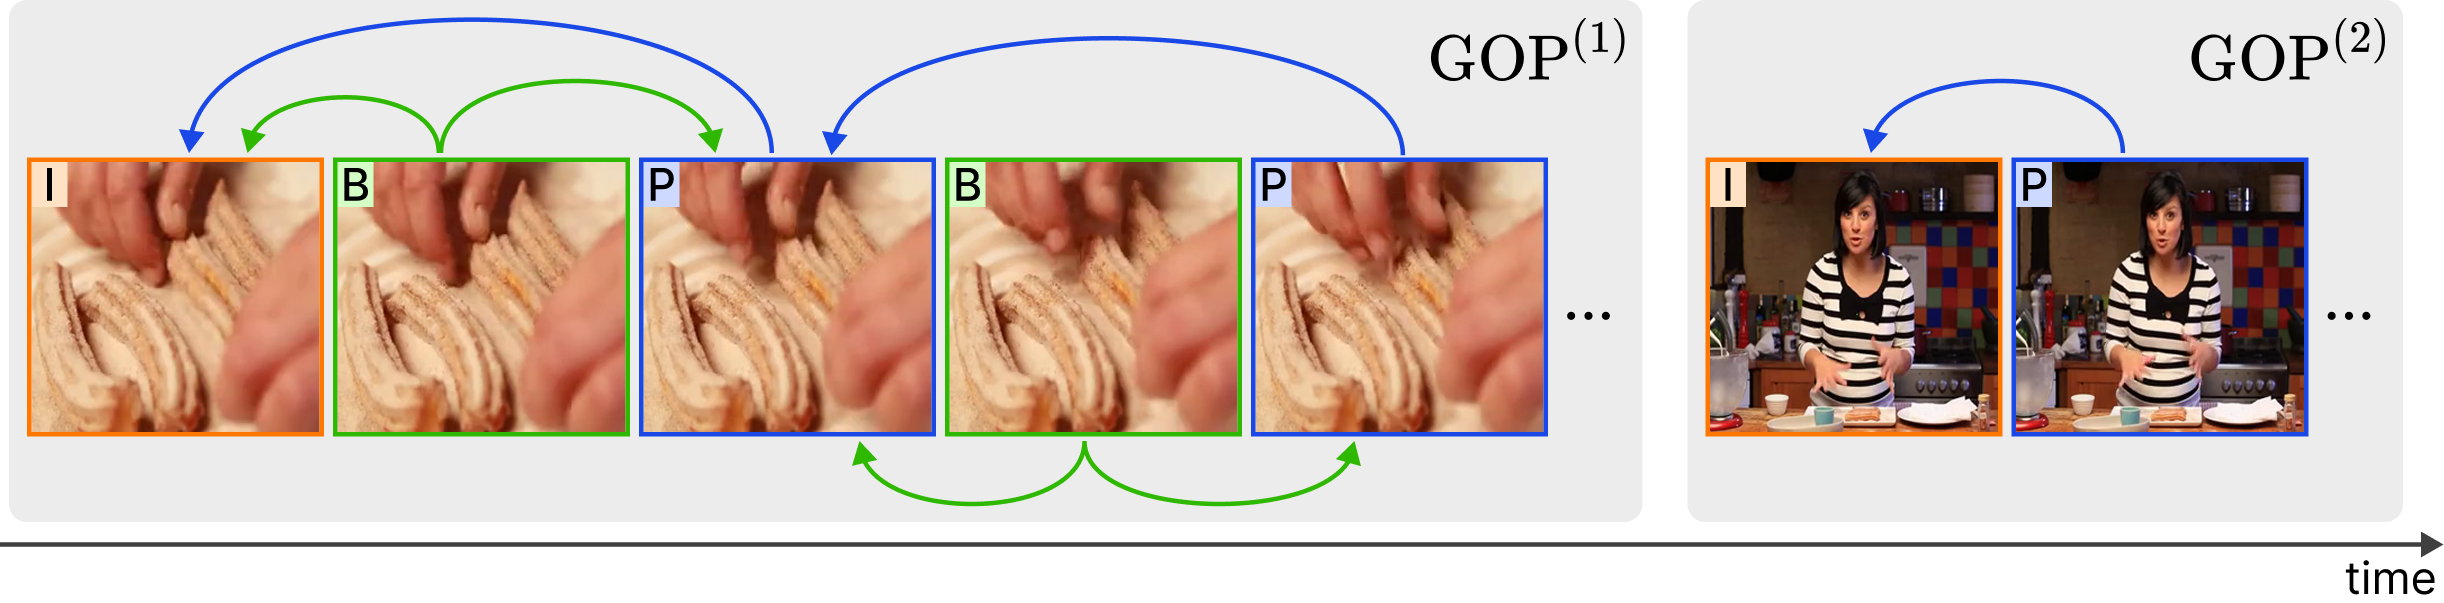
\includegraphics[width=0.99\columnwidth]{figures/fig02_gop_structure.png}
\caption{Illustration of the Group of Pictures (GOP) structure in compressed video. Each GOP begins with an I-frame and includes all subsequent P-frames and B-frames before the next I-frame. Arrows indicate temporal reference dependencies used for inter-frame prediction.}
\label{fig:fig02_gop_structure}
\end{figure}

The GOP structure offers several properties directly relevant to video captioning. First, the I-frame at the beginning of each GOP serves as a natural anchor for extracting appearance and semantic features, given its role as a complete spatial snapshot. Second, the P-frames and B-frames within the same GOP capture short-term temporal dynamics, making them suitable sources for motion feature extraction. Third, because most dependencies remain localized within GOP boundaries, representations extracted from different GOPs tend to contain less redundant temporal information across segments. Together, these properties make GOPs a compact and coherent unit for multimodal video representation.


\subsection{Transformer Building Blocks}
\label{subsec:subsec_32_building_block}
The Transformer architecture is constructed by stacking multiple identical layers composed of attention modules and position-wise feed-forward networks (FFNs), together with residual connections and normalization layers. This section briefly reviews the Transformer building blocks relevant to the proposed model, with particular emphasis on normalization strategies due to their importance for training stability.

% ========== Attention paragraph ==========
At the core of the Transformer is the scaled dot-product attention mechanism, defined as:
\begin{equation}
\mathrm{Attention}(Q,K,V)=\mathrm{Softmax}\left(\frac{QK^T}{\sqrt{d_k}}\right)V,
\end{equation}
where $Q$, $K$, and $V$ denote the query, key, and value representations, respectively, and $d_k$ is the key dimension. To capture information from multiple representation subspaces simultaneously, Transformers employ multi-head attention (MHA):
\begin{align}
\mathrm{MHA}(Q,K,V) &= \mathrm{Concat}(\mathrm{head}_1,\ldots,\mathrm{head}_h)W^O,\\
\mathrm{head}_i &= \mathrm{Attention}(QW_i^Q, KW_i^K, VW_i^V),
\end{align}
where $h$ denotes the number of attention heads, while $W_i^Q, W_i^K, W_i^V$, and $W^O$ are learnable projection matrices. Depending on the sources of $Q$, $K$, and $V$, attention operates either within the same sequence (self-attention) or across different sequences (cross-attention).

% ========== FFN paragraph ==========
Each Transformer layer includes a position-wise FFN consisting of two linear transformations separated by a GELU activation:
\begin{equation}
\mathrm{FFN}(X)=\mathrm{GELU}(XW_1+b_1)W_2+b_2,
\end{equation}
where $W_1$, $W_2$, $b_1$, and $b_2$ are learnable parameters. The FFN is applied independently to each position, providing nonlinear transformation capacity complementary to the attention mechanism.

% ========== 3 LN ==========
\begin{figure}[!t]
\centering
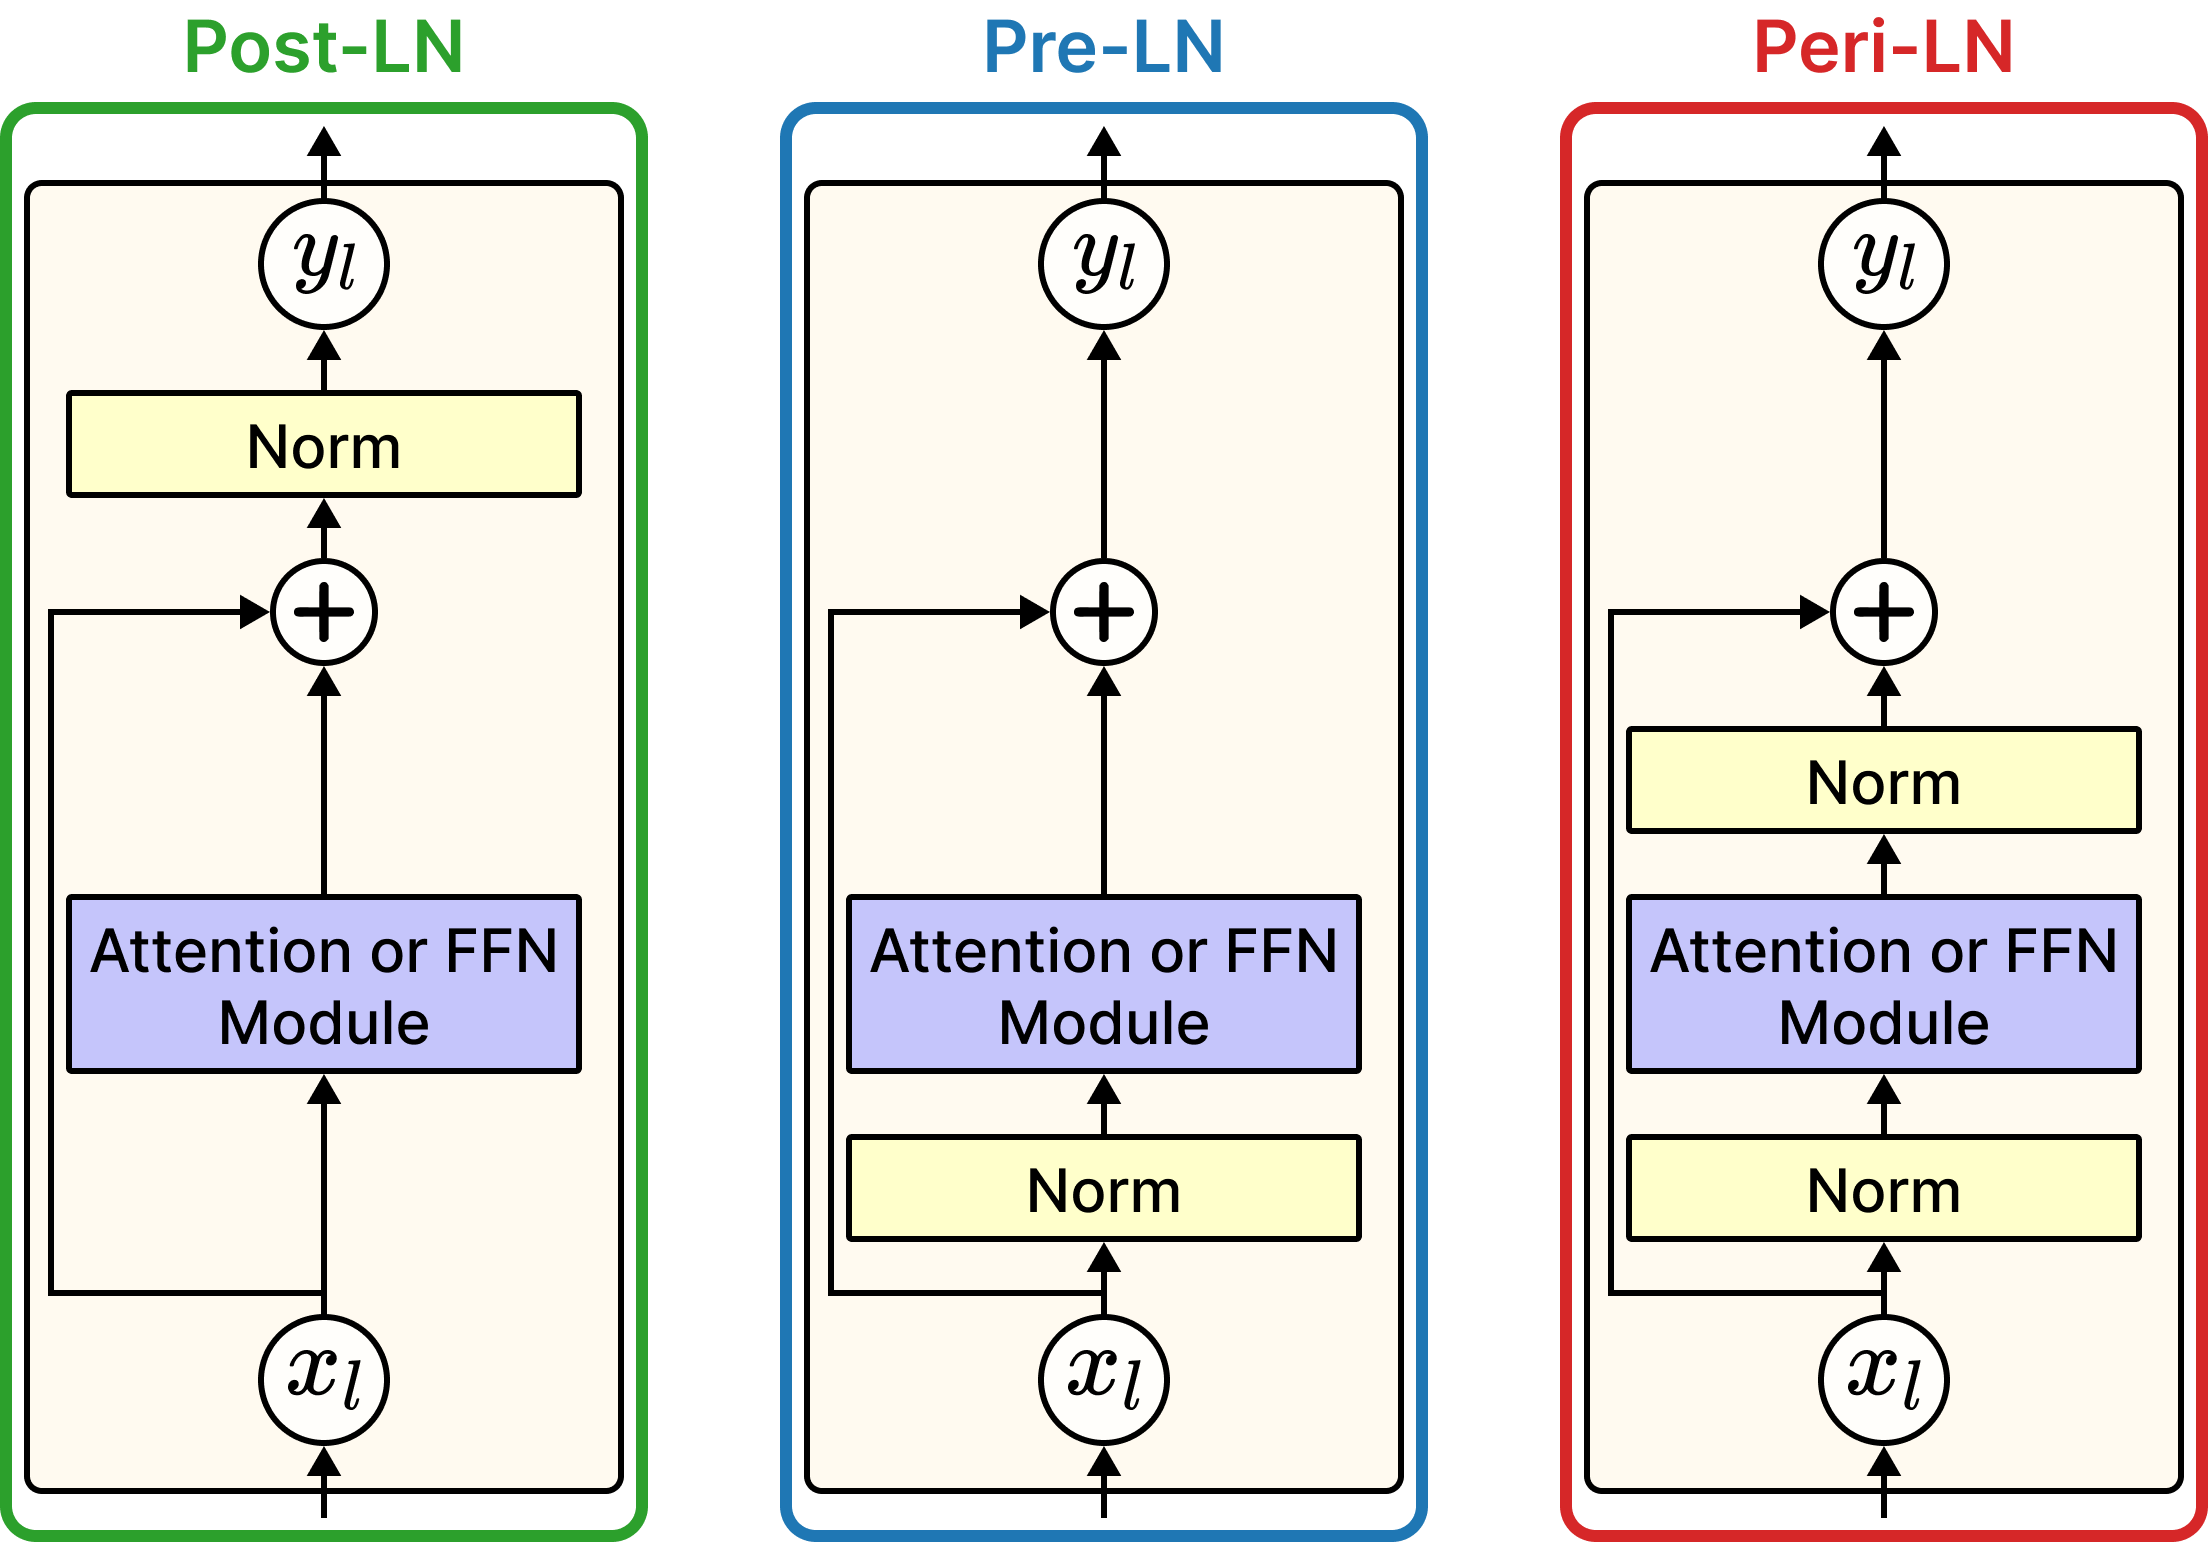
\includegraphics[width=0.90\columnwidth]{figures/fig03_ln_strategies.png}
\caption{Comparison of three layer normalization placement strategies within a Transformer sub-layer. Post-LN applies normalization after residual addition but may weaken gradient propagation in deep networks. Pre-LN improves gradient flow but can lead to hidden-state variance accumulation across layers. Peri-LN addresses both limitations by normalizing both the module input and output, thereby improving training stability.}
\label{fig:fig03_ln_strategies}
\end{figure}


The placement of layer normalization (LN) significantly affects gradient stability and convergence behavior in deep Transformer architectures. Three normalization strategies are particularly relevant to this work. In the original formulation, normalization is applied after residual addition~\cite{vaswaniAttentionAllYou2017}:
\begin{equation}
y_l=\mathrm{Norm}(x_l+\mathrm{Module}(x_l)),
\end{equation}
where $x_l$ and $y_l$ denote the input and output hidden states of the $l$-th sub-layer, respectively, and $\mathrm{Module}(\cdot)$ represents either attention or FFN. Although Post-LN stabilizes hidden-state magnitudes, gradient signals must pass through the normalization layer during backpropagation, which can weaken gradient flow and slow convergence in deep networks~\cite{xiongLayerNormalizationTransformer2020}.

To alleviate the gradient propagation issue of Post-LN, Pre-LN applies normalization before the module operation~\cite{xiongLayerNormalizationTransformer2020}:
\begin{equation}
y_l=x_l+\mathrm{Module}(\mathrm{Norm}(x_l)).
\end{equation}
Pre-LN improves gradient flow during early training. However, because normalization is applied only to the module input, large module outputs can cause hidden-state variance to accumulate across layers, potentially destabilizing optimization in deep networks~\cite{kimPeriLNRevisitingNormalization2025}.

More recent architectures adopt a third strategy, termed \mbox{Peri-LN~\cite{kimPeriLNRevisitingNormalization2025}}, which extends Pre-LN by introducing an additional normalization layer on the module output:
\begin{equation}
y_l=x_l+{\mathrm{Norm}}_{\textit{out}}(\mathrm{Module}({\mathrm{Norm}}_{\textit{in}}(x_l))).
\end{equation}
By normalizing both the input and output of each module, Peri-LN effectively mitigates hidden-state variance accumulation and reduces the risk of excessively large activations, further stabilizing gradient propagation in deep Transformer architectures~\cite{kimPeriLNRevisitingNormalization2025}. Stable normalization becomes particularly important in bidirectional decoding systems, where information flows through both forward and backward contextual pathways. Accordingly, Peri-LN is adopted throughout the proposed architecture. For clarity, normalization layers and residual connections are omitted from subsequent diagrams unless directly relevant to the discussion. Fig.~\ref{fig:fig03_ln_strategies} compares the structures of Post-LN, Pre-LN, and Peri-LN.

